\documentclass[11pt,a4paper]{article}
\usepackage[utf8]{inputenc}
\usepackage[T1]{fontenc}
\usepackage[a4paper]{geometry}

\usepackage{amsthm}
\newtheorem{theo}{Théorème}
\newtheorem{defi}[theo]{Définition}
\newtheorem{prop}[theo]{Proposition}

\usepackage{amssymb}
\usepackage{amsmath}
\usepackage{bbm}
\usepackage{stmaryrd}
\usepackage{proof}
\usepackage{tikz}
\usetikzlibrary{matrix}
\usetikzlibrary{decorations.pathmorphing}

\setlength\parindent{0pt}

\newcommand{\La}{\mathcal{L}}
\newcommand{\M}{\mathcal{M}}
\newcommand{\ph}{\varphi}
\newcommand{\itemz}{\item[$\triangleright$]}
\newcommand{\F}{\mathcal{F}}
\newcommand{\gr}{\textbf}
\newcommand{\il}{\textit}
\newcommand{\N}{\mathbb{N}}
\newcommand{\U}{\mathcal{U}}
\newcommand{\preuve}{\begin{proof}[Preuve]}
\newcommand{\cqfd}{\end{proof}}
\newcommand{\equi}{\Leftrightarrow}
\newcommand{\R}{\mathcal{R}}
\newcommand{\C}{\mathcal{C}}
\newcommand{\I}{\mathcal{I}}
\renewcommand{\iff}{\Leftrightarrow}
\newcommand{\T}{\mathcal{T}}
\newcommand{\V}{\mathcal{V}}
\newcommand{\lb}{\llbracket}
\newcommand{\rb}{\rrbracket}
\newcommand{\info}[1]{\text{{\fontfamily{lmss}\selectfont #1}}}
\newcommand{\Mod}{\info{Mod}}
\newcommand{\Sen}{\info{Sen}}
\renewcommand{\P}{\mathcal{P}}
\newcommand{\1}{\mathbbm{1}}
\renewcommand{\contentsname}{Table des matières}
\renewcommand{\proofname}{Preuve}


\usepackage[bitstream-charter]{mathdesign}
%\usepackage[charter]{mathdesign}
%\usepackage{fontspec}
%\setmainfont{URW Palladio L}



\begin{document}

\section{Ultraproduits en théorie des institutions}

\subsection{Concepts de théorie des catégories}

\begin{defi}[Diagram]
Soit $\gr{I}$ et $\gr{C}$ des catégories. Un diagramme de type $\gr{I}$ est un foncteur $D : \gr{I} \to \gr{C}$.
\end{defi}
\gr{Remarque.} La catégorie $\gr{J}$ est appelée catégorie d'indexation. Ni ses objets, ni ses morphismes n'importent vraiment ; seule la forme de son graphe sera utilisée. Par exemple, soit $\gr{I}$ la catégorie comportant deux objets $A,B$ et un seul morphisme non trivial $f : A \to B$. On la décrira usuellement comme étant la catégorie $ (\circ \rightarrow \circ) $. Définir un diagramme, c'est alors essentiellement remplacer les $\circ$ par des objets de $\gr{C}$. Dans le cas précis où $\gr{I} = (\circ \leftarrow \circ \rightarrow \circ)$, un diagramme de type $\gr{I}$ est appelé un \il{span}. Si on prend $\gr{I} = (\circ \rightarrow \circ \leftarrow \circ)$, il est appelé \il{cospan}.

\begin{defi}[Cone]
Soit $D : \gr{I} \to \gr{C}$ un diagramme. Un cône est un tuple $(C,\psi)$ composé d'un objet $C$ de $\gr{C}$ et d'une famille de morphismes $\psi_i : C \to D(i)$ pour tout objet $i$ de $\gr{I}$, tel que chacun des triangles ci-dessous commute pour tous $i,j$ et tout $f : i \to j$

\begin{center}
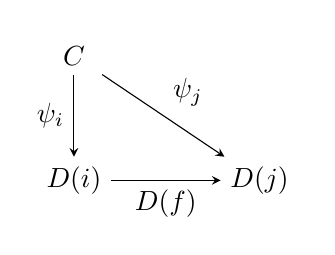
\begin{tikzpicture}
  \matrix (m) [matrix of math nodes,row sep=3em,column sep=4em,minimum width=2em]
  {
     C & \\
     D(i) & D(j) \\};
  \path[-stealth]
    (m-1-1) edge node [left] {$\psi_i$} (m-2-1)
    (m-2-1) edge node [below] {$D(f)$}(m-2-2)
    (m-1-1) edge node [above right] {$\psi_j$} (m-2-2);
\end{tikzpicture}
\end{center}

\end{defi}

\begin{defi}[Produit]
Soit $\gr{C}$ une catégorie et $(X_i)_{i\in I}$ une famille d'objets indexée par un ensemble $I$. Alors l'objet $X$ est le produit de la famille $(X_i)_{i\in I}$ si il existe des morphismes $\pi_i : X \to X_i$ tels que pour tout objet $Y$ et tous morphismes $f_i : Y \to X_i$, il existe un unique morphisme $f : Y \to X$ tel que pour tout $i \in I$ le diagramme suivant commute :

\begin{center}
\begin{tikzpicture}
  \matrix (m) [matrix of math nodes,row sep=3em,column sep=4em,minimum width=2em]
  {
     Y & X \\
      & X_i \\};
  \path[-stealth]
    (m-1-1) edge node [above] {$f$} (m-1-2)
    (m-1-2) edge node [right] {$\pi_i$}(m-2-2)
    (m-1-1) edge node [below left] {$f_i$} (m-2-2);
\end{tikzpicture}
\end{center}
\end{defi}
\gr{Exemples.} 
\begin{itemize}
\item[$\bullet$] Dans $\gr{Set}$, soit $(X_i)_{i\in I}$ des ensembles. On pose $X = \prod_{j\in I} X_j$ le produit cartésien de cette famille. Montrons qu'il s'agit du produit de $(X_i)_{i\in I}$ au sens des catégories, avec $\pi_i : \prod_{j\in I} X_j \to X_i$ la projection canonique. Soit donc un objet $Y$ et des fonctions $f_i : Y \to X_i$. Soit $i \in I$ quelconque, la commutation du diagramme signifie que $f_i(y) = \pi_i(f(y))$. Il est donc équivalent que le diagramme commute pour tout $i \in I$ et que $f(y)_i = f_i(y)$, ce qui donne l'existence et l'unicité de $f$.
\item[$\bullet$] Dans $\gr{Top}$, soit $(X_i,\tau_i)_{i\in I}$ des espaces topologiques. On définit $(X,\tau)$, où $X = \prod_{j\in I} X_j$ et $\tau$ est la plus petite topologie qui rend les projections $\pi_i : \prod_{j\in I} X_j \to X_i$ continues. Montrons que c'est le produit des $(X_i,\tau_i)_{i\in I}$ au sens des catégories. Soit $f_i : Y \to X_i$ des fonctions continues. D'après l'exemple précédent, le seul candidat est $f(y)_i = f_i(y)$. On doit seulement vérifier que définir $f : \prod_{j\in I} X_j$ ainsi en fait une fonction continue. Mais puisque $\pi_i \circ f = f_i$ est continue pour tout $i \in I$ et par définition de $\tau$, c'est automatique.
\end{itemize}

On rappelle la définition d'un filtre.
\begin{defi}[Filtre]
Un filtre sur $I$ est une partie $\F \subseteq \P(I)$ qui vérifie
\begin{enumerate}
\setlength\itemsep{-0.3em}
\item[(i)] $I \in \F$, $\emptyset \notin \F$.
\item[(ii)] Si $X,Y \in \F$ alors $X \cap Y \in \F$ (stabilité par intersections finies).
\item[(iii)] Si $X \subseteq Y$ et $X \in \F$ alors $Y \in \F$.
\end{enumerate}
\end{defi}



\end{document}